% ============================================================
% main_en.tex — Paper English Version
% Title: Safety Zone Characterization in Elderly Hypertensive Patients Using
%        Cardiopulmonary Exercise Testing: A 2×2 HTN×EIH Phenotypic
%        and Machine Learning Classification Study (N=3,206)
%
% Document class: article; Compilation: pdflatex + bibtex
% References: numeric style
%
% Compilation:
%   pdflatex main_en.tex
%   bibtex main_en
%   pdflatex main_en.tex
%   pdflatex main_en.tex
% ============================================================

\documentclass[12pt, a4paper]{article}

% ------ Basic packages ------
\usepackage[utf8]{inputenc}
\usepackage[T1]{fontenc}
\usepackage[english]{babel}
\usepackage{geometry}
\geometry{left=2.5cm, right=2.5cm, top=3cm, bottom=3cm}
\usepackage{setspace}
\onehalfspacing

% ------ References (numeric) ------
\usepackage[numbers,sort&compress]{natbib}
\bibliographystyle{unsrtnat}

% ------ Figures and tables ------
\usepackage{graphicx}
\usepackage{booktabs}
\usepackage{longtable}
\usepackage{array}
\usepackage{makecell}
\usepackage{multirow}
\usepackage{caption}
\captionsetup{font=small, labelfont=bf}

% ------ Math ------
\usepackage{amsmath}
\usepackage{amssymb}

% ------ Color and links ------
\usepackage[dvipsnames]{xcolor}
\usepackage[colorlinks=true, linkcolor=blue, citecolor=blue, urlcolor=blue]{hyperref}

% ------ Other ------
\usepackage{enumitem}
\usepackage{subcaption}
\usepackage{float}
\usepackage{lineno}
% \linenumbers  % Uncomment for review submission

% ------ Metadata ------
\title{\textbf{Safety Zone Characterization in Elderly Hypertensive Patients
Using Cardiopulmonary Exercise Testing:}\\
A 2$\times$2 HTN$\times$EIH Phenotypic and Machine Learning
Classification Study (N=3,206)}

\author{Author Name$^{1}$\\
\small $^{1}$Institution}

\date{April 2026}

% ============================================================
\begin{document}
\maketitle

% ------ Abstract ------
\begin{abstract}
\noindent\textbf{Background:}
Cardiopulmonary exercise testing (CPET) is the gold standard for assessing exercise safety
in cardiovascular patients, yet a systematic safety zone stratification framework for elderly
hypertensive patients remains lacking.

\noindent\textbf{Objectives:}
(1) Characterize CPET phenotypes across hypertension history (HTN) and
exercise-induced hypoxemia (EIH) strata using a 2$\times$2 factorial design;
(2) Develop a dual-timeline safety zone prediction framework (pre-exercise P0 +
post-exercise P1);
(3) Quantify the predictive ceiling of summary-level CPET data with explicit
Leakage Guard protection.

\noindent\textbf{Methods:}
Retrospective single-center study (N=3,206) using a 2$\times$2 design:
HTN history $\times$ EIH response.
Four cohorts: CTRL (n=1,858), HTN-NoEIH (n=738), HTN-EIH (n=277), EIH-Only (n=333).
A 5-layer quality control pipeline with explicit Leakage Guard protection was implemented.
Type II two-way ANOVA (partial $\eta^2$), Dunn's post-hoc comparisons, reference
equations (OLS, n$\approx$968), and Logistic regression for EIH predictors characterized
the phenotypic structure.
Machine learning: P0 (LASSO + XGBoost); P1 (Ordinal Logistic + LightGBM + CatBoost);
SHAP global feature importance.

\noindent\textbf{Results:}
HTN history was the dominant driver of reduced aerobic capacity
(VO$_2$peak $F$=290.6, $p$<0.001, partial $\eta^2$=0.084, medium effect);
EIH response primarily manifested as markedly elevated peak blood pressure
($F$=1803.1, $p$<0.001, $\eta^2$=0.371, large effect).
The HTN$\times$EIH interaction on VO$_2$peak was non-significant ($F$=0.02, $p$=0.894),
indicating independent rather than synergistic effects.
HTN groups showed median VO$_2$peak 19.2--20.1 vs 23.2--23.5 mL/kg/min in non-HTN groups.
Safety zone distribution: Green 40.2\%, Yellow 34.3\%, Red 24.9\%;
HTN-EIH Red zone 99.3\%, CTRL Red zone 6.3\%.
P0: XGBoost AUC=0.583; P1: CatBoost F1$_\text{macro}$=0.499, $\kappa$=0.302;
reflecting summary-level predictive ceiling.
SHAP identified VO$_2$peak and peak heart rate as dominant features.

\noindent\textbf{Conclusions:}
HTN and EIH affect distinct cardiopulmonary dimensions through independent main
effects rather than synergistic interaction.
Summary-level CPET data approaches its predictive ceiling (P0 AUC$\approx$0.58,
P1 F1$\approx$0.50), necessitating breath-by-breath waveform data for further improvement.
The Leakage Guard methodology quantified the leakage effect at $\approx$0.37 F1 units,
providing a reproducible framework for retrospective CPET studies.

\noindent\textbf{Keywords:} Cardiopulmonary exercise testing; Exercise safety;
Hypertension; Exercise-induced hypoxemia; Machine learning; Safety zone
\end{abstract}

\tableofcontents
\newpage

% ============================================================
\section{Introduction}
% ============================================================

Cardiovascular disease (CVD) is the leading cause of mortality and disability in elderly
populations worldwide~\cite{WHO2023}.
Exercise-based cardiac rehabilitation significantly improves cardiopulmonary function and
prognosis~\cite{Piepoli2016,Thomas2019},
yet exercise-induced adverse events---particularly exercise-induced hypoxemia (EIH) and
hypertensive stress responses---remain significant barriers to safe exercise
prescription~\cite{Myers2013,Agostoni2013}.

Cardiopulmonary exercise testing (CPET) provides a comprehensive assessment of
cardiorespiratory reserve and is the gold standard for exercise safety
evaluation~\cite{Balady2010,Guazzi2012}.
However, a systematic CPET-based safety zone classification for elderly hypertensive
patients remains underdeveloped:
(1) the interaction between hypertension history and EIH has not been systematically
quantified in large cohorts;
(2) the predictive ceiling of summary-level CPET data for machine learning is unknown;
(3) data leakage---a pervasive methodological issue in retrospective CPET
modeling---is rarely explicitly addressed~\cite{Ross2024}.

Machine learning applied to CPET data has yielded promising results:
Li et al.~\cite{Li2022xgb} achieved AUC=0.794 in coronary artery disease patients,
Arina et al.~\cite{Arina2025} reached AUC=0.946 in perioperative elderly patients,
but both included extensive clinical laboratory features (medications, echocardiographic
data)~\cite{Hearn2018,Zignoli2022ejss}.
The Chinese CPET expert consensus~\cite{SunXG2022consensus} recommends standardized
CPET protocols, but quantitative safety zone frameworks for elderly hypertensive patients
based on large-scale data remain lacking.

This study aims to:
(1) characterize CPET phenotypes using a HTN$\times$EIH 2$\times$2 design;
(2) develop a dual-timeline safety zone framework (P0 pre-exercise + P1 post-exercise);
(3) establish Leakage Guard methodology to quantify and prevent data leakage in
retrospective CPET modeling.

% ============================================================
\section{Methods}
% ============================================================

\subsection{Study Population and Design}

This retrospective single-center cohort study enrolled patients $\geq$60 years who
completed CPET at our institution from 2015 to 2023.
Of 3,232 eligible records, 3,206 passed quality control (26 excluded, 0.8\%) and were
included in analysis.

A 2$\times$2 factorial design stratified patients by:
\begin{itemize}
    \item Factor A: HTN history (prior diagnosis of hypertension: Yes/No)
    \item Factor B: EIH response (exercise-induced SpO$_2$ drop $\geq$4\% or nadir <90\%: Yes/No)
\end{itemize}

\begin{table}[H]
\centering
\caption{HTN$\times$EIH 2$\times$2 Cohort Design}
\label{tab:cohort}
\begin{tabular}{lccc}
\toprule
Cohort & Code & N (post-QC) & Description \\
\midrule
Control/non-HTN & CTRL & 1,858 & No HTN history, no EIH \\
HTN history, no EIH & HTN-NoEIH & 738 & HTN history, no EIH during test \\
HTN history + EIH & HTN-EIH & 277 & HTN history + EIH during test \\
EIH only & EIH-Only & 333 & No HTN history, EIH during test \\
\midrule
Total & & 3,206 & (3,232 pre-QC) \\
\bottomrule
\end{tabular}
\end{table}

This study was approved by the Institutional Review Board (Approval No.: to be filled).
Data were fully de-identified.

\subsection{CPET Protocol and Variable Definitions}

CPET was performed using an incremental cycling or treadmill protocol with a
standard metabolic gas analysis system.
Key variables: VO$_2$peak (mL/kg/min), HR$_\text{peak}$ (bpm), O$_2$ pulse (mL/beat),
VT1-VO$_2$, VE/VCO$_2$ slope, heart rate recovery at 1 minute (HRR1), oxygen uptake
efficiency slope (OUES), peak METs.

\textbf{EIH definition}: SpO$_2$ drop $\geq$4\% from rest or nadir <90\% during exercise.
In this dataset, EIH was identified from the group\_code field (groups containing ``EHT'').

\subsection{Quality Control Pipeline}

A 5-layer QC pipeline was applied:
(1) physiological range compliance (35 outlier values clipped);
(2) cross-field logical consistency;
(3) missing rate threshold check (>30\% flagged; medication fields entirely absent);
(4) protocol consistency standardization (cycling/treadmill);
(5) EHT\_ONLY group-specific diagnostics (139 missing peak SBP values).

\textbf{Leakage Guard}: Since eih\_status directly participates in P1 zone definition
(P1 Red criterion), and ve\_vco2\_slope and vo2\_peak\_pct\_pred participate in P1 label
construction, an explicit Leakage Guard mechanism was established.
All label-participating fields were forcibly excluded from model features.
This prevented inflated model performance: leaked model F1=0.84 vs.\ clean model F1=0.47,
a leakage effect of $\approx$0.37 F1 units~\cite{Ross2024,Lundberg2017}.

\subsection{Safety Zone Definitions}

A dual-timeline design was adopted:

\textbf{P0 (pre-exercise prediction of exercise-induced adverse events, binary)}:
P0 labels are defined by exercise-derived measurements, while the P0 model uses only
pre-exercise baseline information (age, sex, BMI, medical history, etc.)
to predict whether adverse events will occur during or after exercise.
This constitutes a prospective prediction task despite the retrospective study design,
with strict separation between feature time-point (pre-exercise) and label time-point (during/post-exercise).
Positive if any criterion is met:
(1) eih\_status = True (SpO$_2$ drop $\geq$4\% or absolute $<$90\% during exercise);
(2) VO$_2$peak $<$50\% predicted (post-exercise);
(3) Peak SBP $>$220 mmHg (during exercise).

\textbf{P1 (post-exercise safety zone stratification, 3-class ordinal)}:
P1 is defined using three exercise-derived variables and employs a take-worst strategy
(most severe zone assigned when criteria conflict):
\begin{itemize}
    \item \textbf{Green (low risk)}: eih\_status = False,
          AND VO$_2$peak $\geq$70\% predicted, AND VE/VCO$_2$ slope $\leq$30
    \item \textbf{Yellow (moderate risk)}: eih\_status = False,
          AND (VO$_2$peak 50--70\% OR VE/VCO$_2$ slope 30--36; not meeting Green/Red criteria)
    \item \textbf{Red (high risk)}: eih\_status = True (independent sufficient condition),
          OR VO$_2$peak $<$50\% predicted, OR VE/VCO$_2$ slope $>$36
\end{itemize}

\begin{quote}
\textbf{Note (Label Construction Axiom)}: EIH positivity (eih\_status = True) is an independent
sufficient condition for Red zone assignment — EIH$+$ patients are axiomatically classified
as Red regardless of VO$_2$peak or VE/VCO$_2$ values. This reflects clinical consensus
that EIH constitutes a high-risk marker~\cite{SunXG2022consensus}.
Consequently, the near-100\% Red proportion in EIH$+$ cohorts is a structural consequence
of the label definition, not a model prediction.
The Leakage Guard mandatorily excludes eih\_status from P1 model features,
ensuring the model cannot exploit this axiomatic constraint;
P1 model predictions are meaningful for non-EIH patients.
\end{quote}

\subsection{Statistical Analysis}

Baseline characteristics: Kruskal-Wallis test (non-normal continuous variables) and
$\chi^2$ test (categorical variables); Dunn's post-hoc pairwise comparisons with
Bonferroni correction ($\alpha$=0.0083 for 6 pairs).

HTN$\times$EIH interaction: Type II two-way ANOVA with partial $\eta^2$
(negligible $<$0.01, small 0.01--0.06, medium 0.06--0.14, large $\geq$0.14, per Cohen 1988)~\cite{Cohen1988}.
Given the large sample size (N=3,206), even negligible effects ($\eta^2<0.01$) can reach statistical significance.
Effect sizes ($\eta^2$) rather than $p$-values serve as the primary interpretation criterion;
effect size categories are indicated in table footnotes ($^n/^s/^m/^L$).

Reference equations: OLS regression on reference-normal subset with
age, sex, and age$\times$sex interaction as predictors, outputting \%predicted and z-scores.

EIH predictors: Univariable and multivariable Logistic regression.

\subsection{Machine Learning Models}

\textbf{P0 models}: LASSO logistic regression (baseline, L1 regularization) and
XGBoost (primary model).
5-fold cross-validation with isotonic calibration.
Metrics: AUC-ROC, AUPRC, Brier score.

\textbf{P1 models}: Ordinal logistic (baseline), LightGBM (primary), CatBoost (comparison).
Ordinal 3-class output (green=0/yellow=1/red=2), class-balanced training.
Metrics: F1$_\text{macro}$, Cohen's $\kappa$, per-class recall.

\textbf{Cost-sensitive sensitivity analysis}: LightGBM with Red class weight$\times$4,
quantifying the F1-vs-safety trade-off~\cite{Hastie2009}.

Feature importance: SHAP (SHapley Additive exPlanations)~\cite{Lundberg2017}.

% ============================================================
\section{Results}
% ============================================================

\subsection{Baseline Characteristics}

Baseline characteristics are presented in Table~\ref{tab:table1}.
The median age across all cohorts was 67 years with no significant difference ($p$=0.375).
HTN groups (HTN-NoEIH and HTN-EIH) had significantly higher body weight than
non-HTN groups ($p$<0.001), consistent with metabolic comorbidities in hypertension.
HTN-NoEIH showed the lowest median VO$_2$peak (19.2 mL/kg/min),
while EIH-Only showed the highest (23.5 mL/kg/min).
HTN-EIH had the highest median peak SBP (214 mmHg).
Post-hoc analysis (Dunn's, Bonferroni corrected) identified significant pairwise
differences in 10 of 11 key variables.

\begin{table}[H]
\centering
\small
\caption{Baseline characteristics by 2$\times$2 cohort (Table 1)}
\label{tab:table1}
\begin{tabular}{lccccc}
\toprule
Variable & CTRL & HTN-NoEIH & HTN-EIH & EIH-Only & $P$ \\
 & (n=1,858) & (n=738) & (n=277) & (n=333) & \\
\midrule
\multicolumn{6}{l}{\textit{Continuous variables (median [Q1,Q3])}} \\
Age (years) & 67 [63,72] & 67 [63,71] & 67 [63,71] & 67 [64,71] & 0.375 \\
VO$_2$peak (mL/kg/min) & 23.2 [19.5,28.3] & 19.2 [16.2,23.0] & 20.1 [16.8,23.4] & 23.5 [19.3,28.9] & <0.001 \\
VO$_2$peak \%pred (\%) & 77 [66,88] & 72 [62,86] & 80 [67,91] & 79 [68.5,92] & <0.001 \\
HR$_\text{peak}$ (bpm) & 154 [140,167] & 134 [119,148] & 145 [129,158] & 158 [145,170] & <0.001 \\
Peak SBP (mmHg) & 161 [144,178] & 171 [155,184] & 214 [204,226] & 212 [200,223] & <0.001 \\
VE/VCO$_2$ slope & 26.7 [24.2,29.4] & 27.8 [25.3,30.8] & 27.6 [24.8,30.0] & 27.4 [24.4,30.0] & <0.001 \\
O$_2$ pulse (mL/beat) & 10.0 [8.0,13.0] & 10.0 [8.2,13.0] & 10.0 [8.0,13.0] & 11.0 [8.0,14.0] & 0.036 \\
\midrule
\multicolumn{6}{l}{\textit{Categorical variables (n, \%)}} \\
Female & 926 (49.8\%) & 312 (42.3\%) & 135 (48.9\%) & 147 (44.1\%) & 0.004 \\
HTN history & 0 (0\%) & 738 (100\%) & 277 (100\%) & 0 (0\%) & <0.001 \\
EIH (exercise HTN) & 0 (0\%) & 0 (0\%) & 277 (100\%) & 333 (100\%) & <0.001 \\
\bottomrule
\end{tabular}
\\[1ex]
\footnotesize Continuous: Kruskal-Wallis; categorical: $\chi^2$. Dunn's post-hoc: 10/11 variables with significant pairwise differences. Diabetes and comorbidity fields were entirely absent in the current dataset.
\end{table}

\subsection{HTN$\times$EIH Interaction Effects (Two-way ANOVA)}

Results of Type II two-way ANOVA are presented in Table~\ref{tab:anova}.

\begin{table}[H]
\centering
\small
\caption{HTN$\times$EIH two-way ANOVA results (Table 2)}
\label{tab:anova}
\begin{tabular}{lcccccccc}
\toprule
\multirow{2}{*}{Outcome} & \multicolumn{3}{c}{HTN main effect} & \multicolumn{3}{c}{EIH main effect} & \multicolumn{2}{c}{Interaction (A$\times$B)} \\
\cmidrule(lr){2-4}\cmidrule(lr){5-7}\cmidrule(lr){8-9}
 & $F$ & $p$ & $\eta^2$ & $F$ & $p$ & $\eta^2$ & $F$ ($p$) & $\eta^2$ \\
\midrule
VO$_2$peak & 290.6 & <0.001 & 0.084$^m$ & 4.37 & 0.037 & 0.001$^n$ & 0.02 (0.894) & 0.000$^n$ \\
VO$_2$peak \%pred & 22.3 & <0.001 & 0.007$^n$ & 25.9 & <0.001 & 0.008$^n$ & 5.03 (0.025) & 0.002$^n$ \\
HR$_\text{peak}$ & 487.6 & <0.001 & 0.133$^m$ & 42.4 & <0.001 & 0.013$^s$ & 12.87 (<0.001) & 0.004$^n$ \\
Peak SBP & 65.6 & <0.001 & 0.021$^s$ & 1803.1 & <0.001 & 0.371$^L$ & 5.20 (0.023) & 0.002$^n$ \\
VE/VCO$_2$ slope & 38.2 & <0.001 & 0.012$^s$ & 0.34 & 0.558 & 0.000$^n$ & 3.37 (0.067) & 0.001$^n$ \\
O$_2$ pulse & 2.91 & 0.088 & 0.001$^n$ & 9.67 & 0.002 & 0.003$^n$ & 5.84 (0.016) & 0.002$^n$ \\
\bottomrule
\end{tabular}
\\[1ex]
\footnotesize Effect size: $^n$ negligible ($<$0.01), $^s$ small (0.01--0.06), $^m$ medium (0.06--0.14), $^L$ large ($>$0.14) (Cohen 1988).
\end{table}

Key findings (Figure~\ref{fig:interaction}):
HTN history significantly reduced VO$_2$peak ($\eta^2$=0.084, medium effect) and HR$_\text{peak}$
($\eta^2$=0.133, medium effect).
EIH response primarily drove a large increase in peak SBP ($\eta^2$=0.371, large effect;
cell means: EIH$+$ 213 vs.\ EIH$-$ 163 mmHg), with negligible independent effect on VO$_2$peak.
The HTN$\times$EIH interaction on VO$_2$peak was non-significant ($F$=0.02, $p$=0.894, $\eta^2$=0.000).
Although some interaction effects reached statistical significance in this large sample
(VO$_2$peak\%pred: $p$=0.025; HR$_\text{peak}$: $p$<0.001; peak SBP: $p$=0.023),
all interaction $\eta^2$ values were negligible ($\leq$0.004), indicating no clinically meaningful
synergistic interaction between HTN and EIH.
The two factors operate through independent main effects on distinct cardiopulmonary dimensions.

\subsection{Reference Equations}

The reference-normal subset (n$\approx$968, 479 male, 489 female) yielded reference
equations for five key CPET variables (Table~\ref{tab:refequations}).

\begin{table}[H]
\centering
\small
\caption{Reference normal equations (Table 3)}
\label{tab:refequations}
\begin{tabular}{lccl}
\toprule
Variable & N & $R^2$ & Key coefficients \\
\midrule
VO$_2$peak (mL/kg/min) & 968 & 0.298 & Intercept=29.38; age coeff=$-$0.092; sex$\times$age interaction \\
VO$_2$peak \%pred (\%) & 969 & 0.013 & Limited predictability from age/sex \\
HR$_\text{peak}$ (bpm) & 966 & 0.082 & Intercept=134.5; age coeff=+0.257 \\
VE/VCO$_2$ slope & 969 & 0.040 & Intercept=30.5; age coeff=$-$0.067 \\
O$_2$ pulse (mL/beat) & 968 & 0.489 & Intercept=11.37; age coeff=$-$0.032 \\
\bottomrule
\end{tabular}
\\[1ex]
\footnotesize All models include age, sex (M/F), and age$\times$sex interaction. VO$_2$peak $R^2$=0.298 indicates substantial individual heterogeneity in the elderly population (residual SD=6.3 mL/kg/min). O$_2$ pulse $R^2$=0.489 reflects the strong body-size dependence of stroke volume.
\end{table}

\subsection{Safety Zone Distribution}

Overall zone distribution (Figure~\ref{fig:zone_dist}):
Green 1,289 (40.2\%), Yellow 1,099 (34.3\%), Red 797 (24.9\%), missing 21 (0.7\%).

Distribution by 2$\times$2 cohort:
\begin{itemize}
    \item HTN-EIH (n=277): Red 275 (\textbf{99.3\%}), Green/Yellow 0
    \item EIH-Only (n=333): Red 324 (\textbf{97.3\%}), Green/Yellow 0
    \item HTN-NoEIH (n=738): Green 299 (40.5\%), Yellow 353 (47.8\%), Red 81 (11.0\%)
    \item CTRL (n=1,858): Green 990 (53.3\%), Yellow 746 (40.2\%), Red 117 (\textbf{6.3\%})
\end{itemize}

P0 event rate: 727/3,206 (22.7\%).
P0 trigger breakdown: EIH 610 (19.0\%), VO$_2$peak$<$50\%pred 133 (4.1\%),
peak SBP$>$220 mmHg 146 (4.6\%) (triggers may overlap).

\noindent\textbf{Note (EIH-Red Axiomatic Constraint)}:
The near-100\% Red proportions in HTN-EIH (99.3\%) and EIH-Only (97.3\%) groups
are an axiomatic consequence of the P1 label definition (eih\_status = True is an
independent sufficient condition for Red), not a model prediction result (see Section~2.4).
Model predictions are meaningful only for non-EIH patients;
the P1 zone for EIH$+$ patients is predetermined by the label construction rule.
The few EIH$+$ cases not assigned Red (0 in HTN-EIH; 9 in EIH-Only) had missing eih\_status values
(NaN does not trigger the EIH-Red condition).

\subsection{P0 Pre-exercise Risk Prediction}

P0 model performance is summarized in Table~\ref{tab:p0models}.

\begin{table}[H]
\centering
\small
\caption{P0 pre-exercise risk model comparison (Table 4)}
\label{tab:p0models}
\begin{tabular}{llccccc}
\toprule
Model & Variant & AUC-ROC & AUPRC & Brier & CV-AUC (mean$\pm$SD) \\
\midrule
LASSO & with BP & 0.582 & 0.284 & 0.174 & 0.622$\pm$0.030 \\
LASSO & no BP & 0.582 & 0.284 & 0.174 & 0.622$\pm$0.030 \\
XGBoost & with BP & 0.583 & 0.287 & 0.180 & 0.623$\pm$0.028 \\
\textbf{XGBoost} & \textbf{no BP} & \textbf{0.583} & \textbf{0.287} & \textbf{0.180} & \textbf{0.623$\pm$0.028} \\
\bottomrule
\end{tabular}
\\[1ex]
\footnotesize LeakageGuard validated (pass). Resting BP data were absent in all records; with-BP and no-BP variants yield identical results. P0 AUC$\approx$0.58 is attributable to absence of medication data (30 fields, all zero), missing resting hemodynamics, and LVEF.
\end{table}

The ROC curve is shown in Figure~\ref{fig:p0_roc}.
SHAP analysis (Figure~\ref{fig:shap_p0}) identified age and HTN history as the most
important predictors.

\subsection{P1 Post-exercise Safety Zone Classification}

P1 model performance is summarized in Table~\ref{tab:p1models}.

\begin{table}[H]
\centering
\small
\caption{P1 post-exercise safety zone classification (Table 5)}
\label{tab:p1models}
\begin{tabular}{llccccc}
\toprule
Model & Sample & F1$_\text{macro}$ & $\kappa$ & Accuracy & CV-F1 (mean$\pm$SD) \\
\midrule
Ordinal Logistic & full & 0.386 & 0.225 & 0.504 & 0.393$\pm$0.013 \\
LightGBM & full & 0.465 & 0.258 & 0.499 & 0.460$\pm$0.007 \\
\textbf{CatBoost} & \textbf{full} & \textbf{0.499} & \textbf{0.302} & \textbf{0.528} & \textbf{0.447$\pm$0.015} \\
\bottomrule
\end{tabular}
\\[1ex]
\footnotesize Cycling-only vs.\ full-sample results were identical (exercise\_protocol field entirely unknown). Best model: CatBoost with F1$_\text{macro}$=0.499, Cohen's $\kappa$=0.302.
\end{table}

Confusion matrix analysis (Figure~\ref{fig:p1_cm}, CatBoost):
Green recall 67.1\% (173/258), Yellow recall 51.8\% (114/220),
Red recall 30.8\% (49/159).

SHAP analysis (Figure~\ref{fig:shap_p1}) identified VO$_2$peak and HR$_\text{peak}$
as the most important classification features.

\textbf{Cost-sensitive sensitivity analysis} (Table~\ref{tab:cost_sensitive}):

\begin{table}[H]
\centering
\small
\caption{Cost-sensitive vs.\ standard model comparison (Table 6)}
\label{tab:cost_sensitive}
\begin{tabular}{lccccc}
\toprule
Model & F1$_\text{macro}$ & $\kappa$ & Green Recall & Yellow Recall & Red Recall \\
\midrule
LightGBM (standard) & 0.465 & 0.258 & — & — & 23.9\% (38/159) \\
\textbf{LightGBM (CS, Red$\times$4)} & \textbf{0.392} & \textbf{0.128} & — & — & \textbf{53.5\% (85/159)} \\
CatBoost (standard) & 0.499 & 0.302 & 67.1\% & 51.8\% & 30.8\% \\
CatBoost (CS) & 0.187 & 0.023 & — & — & 96.2\% (collapsed) \\
\bottomrule
\end{tabular}
\\[1ex]
\footnotesize CS = cost-sensitive; Red$\times$4 = Red class weight 4$\times$. LightGBM CS trades F1 ($-$0.07) for Red recall (+29.6\%); CatBoost CS collapses to predicting Red for all.
\end{table}

\subsection{P1 Proxy Leakage Ablation}

To quantify the proxy leakage contribution of \texttt{vo2\_peak} (absolute value)
toward reconstructing the \texttt{vo2\_peak\_pct\_pred} threshold in P1 zone labels,
a three-variant ablation study was conducted (Table~\ref{tab:ablation}).

\begin{table}[H]
\centering
\small
\caption{P1 proxy leakage ablation study (Table 8)}
\label{tab:ablation}
\begin{tabular}{llccccc}
\toprule
Variant & Feature set & F1$_\text{macro}$ & $\kappa$ & Green Rec. & Yellow Rec. & Red Rec. \\
\midrule
Full & All P1 features (incl.\ vo2\_peak) & 0.458 & 0.237 & 0.630 & 0.481 & 0.268 \\
No-VO2 & Exclude vo2\_peak & 0.455 & 0.243 & 0.627 & 0.481 & 0.261 \\
VO2-only & Only vo2\_peak + age + sex & 0.441 & 0.200 & 0.612 & 0.476 & 0.242 \\
\bottomrule
\end{tabular}
\\[1ex]
\footnotesize Full vs.\ No-VO2: $\Delta$F1=+0.003 (negligible); VO2-only (leakage upper bound) F1=0.441.
\end{table}

The Full vs.\ No-VO2 F1 difference (0.003) is negligible, indicating that
\texttt{vo2\_peak} absolute values have limited capacity to proxy the label threshold
in this dataset. The primary reason is the low predictive power of the reference equation
($R^2$=0.298), which limits the model's ability to reconstruct \texttt{vo2\_peak\_pct\_pred}
from \texttt{vo2\_peak} + age + sex. The leakage upper bound (VO2-only, F1=0.441)
also falls below Full (F1=0.458), confirming that the P1 F1$\approx$0.50 ceiling
reflects inherent feature set limitations rather than leakage-driven inflation.

\subsection{EIH Independent Predictors}

Multivariable Logistic regression (Table~\ref{tab:eih_logistic}, Figure~\ref{fig:eih_forest})
identified HTN history (aOR=1.441, $p$<0.001), BMI (aOR=1.585, $p$<0.001),
and female sex (aOR=0.862, $p$=0.005) as independent EIH predictors.
The positive association of VO$_2$peak with EIH after adjustment (aOR=1.230, $p$<0.001)
may reflect exercise intensity selection bias.

\begin{table}[H]
\centering
\small
\caption{EIH independent predictors --- Logistic regression (Table 7)}
\label{tab:eih_logistic}
\begin{tabular}{lcccc}
\toprule
\multirow{2}{*}{Variable} & \multicolumn{2}{c}{Univariable} & \multicolumn{2}{c}{Multivariable} \\
\cmidrule(lr){2-3}\cmidrule(lr){4-5}
 & OR (95\% CI) & $p$ & aOR (95\% CI) & $p$ \\
\midrule
Age & 0.942 (0.865--1.028) & 0.185 & 0.975 (0.896--1.062) & 0.590 \\
Female sex & 1.003 (0.916--1.091) & 0.949 & 0.862 (0.766--0.953) & 0.005 \\
VO$_2$peak & 0.979 (0.880--1.064) & 0.658 & 1.230 (1.109--1.346) & $<$0.001 \\
HTN history & 1.410 (1.306--1.532) & $<$0.001 & 1.441 (1.315--1.606) & $<$0.001 \\
BMI & 1.603 (1.399--1.828) & $<$0.001 & 1.585 (1.366--1.843) & $<$0.001 \\
HTN duration (years) & 1.132 (1.049--1.236) & 0.003 & 0.930 (0.832--1.012) & 0.154 \\
\bottomrule
\end{tabular}
\\[1ex]
\footnotesize N=3,206, EIH positive rate=19.0\% (610/3,206); multivariable model converged.
\end{table}

% ============================================================
\section{Discussion}
% ============================================================

\subsection{Main Findings}

This study provides the first large-scale systematic characterization of CPET safety
zone distributions in elderly hypertensive patients using a HTN$\times$EIH 2$\times$2
factorial design ($N$=3,206). Three key findings emerge:

\textbf{First, HTN and EIH affect distinct cardiopulmonary dimensions through
independent main effects.}
HTN history demonstrated a medium-sized negative effect on aerobic capacity
(VO$_2$peak $\eta^2$=0.084) and chronotropic response (HR$_\text{peak}$ $\eta^2$=0.133).
EIH, by contrast, primarily manifested as a large elevation in peak blood pressure
($\eta^2$=0.371), with negligible independent effect on VO$_2$peak.
Crucially, the VO$_2$peak interaction was non-significant ($F$=0.02, $p$=0.894, $\eta^2$=0.000).
Although VO$_2$peak\%pred ($p$=0.025), HR$_\text{peak}$ ($p$<0.001), and peak SBP ($p$=0.023)
reached statistical significance for interaction terms, all interaction $\eta^2$ values were
negligible ($\leq$0.004), indicating no clinically meaningful synergistic impairment.
This corrects the intuitive assumption of additive aerobic deterioration in HTN-EIH patients~\cite{Ntalianis2024}.
The large sample (N=3,206) amplifies detection of trivial effects; effect size ($\eta^2$) rather
than $p$-values is the appropriate interpretation criterion.

\textbf{Second, the summary-level predictive ceiling is clearly quantified.}
P0 AUC$\approx$0.58 and P1 F1$\approx$0.50 represent the approximate ceiling
achievable from CPET summary-level data.
The primary constraints are: (a) complete absence of medication data
($\beta$-blockers critically affect CPET interpretation); (b) missing resting
hemodynamics (BP, HR, LVEF); (c) the structural EIH-Red axiom
(EIH$+$ patients are by definition Red, yet eih\_status must be excluded to prevent
leakage, creating an irreducible feature-label information gap).

\textbf{Third, the Leakage Guard framework provides a reproducible benchmark.}
The explicit quantification of leakage effect ($\approx$0.37 F1 units: leaked F1=0.84
vs.\ clean F1=0.47) provides a concrete reference for retrospective CPET modeling.
This gap underscores the importance of systematic leakage audit, particularly for
CPET data where test-derived variables often participate in outcome definitions.

\subsection{Comparison with Literature}

Our P0 AUC=0.583 is lower than Li et al.~\cite{Li2022xgb} (AUC=0.794 in CAD patients)
and Arina et al.~\cite{Arina2025} (AUC=0.946 in perioperative elderly patients).
These differences are expected given feature richness: both studies included medications,
echocardiographic parameters (LVEF), and laboratory biomarkers---categories entirely
absent in our dataset.
Rather than a methodological failure, our result defines the performance envelope of
pure summary-level CPET data without ancillary clinical information.

Hearn et al.~\cite{Hearn2018} and Zignoli et al.~\cite{Zignoli2022ejss} demonstrated
that deep learning applied to breath-by-breath CPET waveforms substantially improves
ventilatory threshold detection accuracy, supporting our Stage II plan to incorporate
raw breath-by-breath data.

Our safety zone definition is broadly consistent with the Chinese CPET expert
consensus~\cite{SunXG2022consensus} in using VO$_2$peak \%predicted and VE/VCO$_2$ slope
as primary stratification variables.
Our data provide large-scale evidence supporting the consensus recommendation that
EIH should be considered a high-risk indicator (99.3\% Red rate in HTN-EIH;
97.3\% in EIH-Only).

\subsection{Methodological Contributions}

The \textbf{dual-timeline P0/P1 design} formally separates pre-exercise risk assessment
(P0, using only pre-test variables) from post-exercise stratification (P1, using full CPET
results).
This design, enforced at the code level through Leakage Guard, ensures that P0 models
can be applied in a clinically meaningful way: to screen patients before CPET and
identify those requiring closer monitoring.

The \textbf{Leakage Guard methodology} addresses a systematic gap in retrospective CPET
modeling~\cite{Ross2024}: the coincidence of EIH classification in both label definition
and potential features.
By pre-specifying excluded fields and reporting the leakage effect size, we provide a
framework reproducible in future studies.

\subsection{Clinical Utility and Model Positioning}

\textbf{P0 clinical utility} (Table~\ref{tab:clinical_utility_p0}):
Surprisingly, a 2-variable baseline model (HTN history + BMI) achieved AUC=0.611,
outperforming XGBoost with all features (AUC=0.577, $\Delta$AUC=$-$0.034).
This finding reinforces the ``summary-level predictive ceiling'' narrative:
complex ML models offer no incremental discriminative value over simple clinical rules
when medication, hemodynamic, and laboratory features are absent.
Despite this, P0 demonstrates clinical utility as a \textbf{rule-out tool}:
at the optimal threshold (0.141), NPV=0.853 (when the model predicts low-risk,
85.3\% are truly low-risk), with a net benefit advantage over treat-all strategy
at both 10\% and 20\% decision thresholds.

\begin{table}[H]
\centering
\small
\caption{P0 clinical utility summary (Table 9, optimal threshold 0.141)}
\label{tab:clinical_utility_p0}
\begin{tabular}{lcccc}
\toprule
Model & AUC & NPV & NNS & Net Benefit ($\geq$ Treat-All) \\
\midrule
2-var baseline (HTN + BMI) & 0.611 & — & — & — \\
XGBoost (all features) & 0.577 & 0.853 & 3.8 & Yes (at 10\%--20\% thresholds) \\
\bottomrule
\end{tabular}
\\[1ex]
\footnotesize NPV=Negative Predictive Value; NNS=Number Needed to Screen per true positive.
\end{table}

\textbf{P1 clinical utility}:
Red zone NPV=0.781 (when model predicts ``non-Red'', 78.1\% are truly non-Red),
but dangerous Red$\rightarrow$Green misclassification rate is 29.4\% (45/153 true-Red
patients predicted as Green).
Notably, a simple VO$_2$peak threshold rule ($<$20.1 mL/kg/min) achieves higher Red
recall (48.4\%) than LightGBM (26.8\%), consistent with the predictive ceiling:
in the high-Red-recall clinical scenario, a simple threshold may outperform
complex models constrained by summary-level features.

Based on the above analysis, the clinical value of the P0/P1 models resides in:
(1) \textbf{Methodological framework validation}---the HTN$\times$EIH 2$\times$2 design
with Leakage Guard provides a reproducible analytical paradigm;
(2) \textbf{Feature importance discovery}---SHAP results identify VO$_2$peak and HR$_\text{peak}$
as primary drivers, informing Stage II feature selection;
(3) \textbf{Baseline benchmark}---current performance (P0 AUC=0.583, P1 F1=0.499)
quantifies the summary-level ceiling against which Stage II/III improvements can be measured.
\textbf{Direct clinical deployment is not recommended} at current performance levels.

\subsection{Limitations}

(1) Single-center retrospective design with potential selection bias; no external
validation cohort.
(2) Medication data entirely absent (30 fields all zero), including $\beta$-blockers
that critically affect heart rate and CPET interpretation.
(3) EIH defined from group code derivation rather than continuous SpO$_2$ monitoring,
introducing classification error.
(4) Summary-level CPET data only; breath-by-breath waveforms not available.
(5) The EIH$+$ 100\% Red proportion is a structural axiom of the P1 label definition,
not a model prediction; subgroup performance in EIH$+$ patients does not reflect
real predictive ability.
(6) Reference equation VO$_2$peak $R^2$=0.298 suggests high individual heterogeneity
in the elderly population; \%pred thresholds may require population-specific calibration.

\subsection{Future Directions}

Stage II will incorporate breath-by-breath gas exchange and 12-lead ECG waveforms,
expected to surpass the summary-level ceiling~\cite{Hearn2018,Zignoli2022ejss}.
Stage III will explore whether wearable devices (e.g., Apple Watch) can serve as home
proxies for CPET anchors~\cite{Gao2026}, enabling a home exercise safety corridor
($C_\text{home}$).
Prospective multicenter validation incorporating medication records and resting
hemodynamics is planned.

% ============================================================
\section{Conclusions}
% ============================================================

We established the first CPET-based exercise safety zone stratification framework for elderly
hypertensive patients using an HTN$\times$EIH 2$\times$2 design ($N$=3,206).
Key conclusions:
(1) HTN and EIH affect distinct cardiopulmonary dimensions through independent main
effects---HTN reduces aerobic reserve while EIH amplifies blood pressure stress response;
the HTN$\times$EIH interaction on VO$_2$peak is non-significant;
(2) Summary-level CPET data approaches its predictive ceiling (P0 AUC=0.583,
P1 F1=0.499), establishing the need for breath-by-breath waveform data in Stage II;
(3) The Leakage Guard mechanism quantified the data leakage effect at $\approx$0.37 F1
units, providing a reproducible methodology for preventing data leakage in retrospective
CPET modeling.
This framework establishes laboratory anchor points for subsequent breath-by-breath
modeling and home exercise safety corridor research.

% ============================================================
% References
% ============================================================
\bibliography{references}

% ============================================================
% Figure Captions
% ============================================================
\clearpage
\section*{Figure Captions}

\begin{figure}[H]
\centering
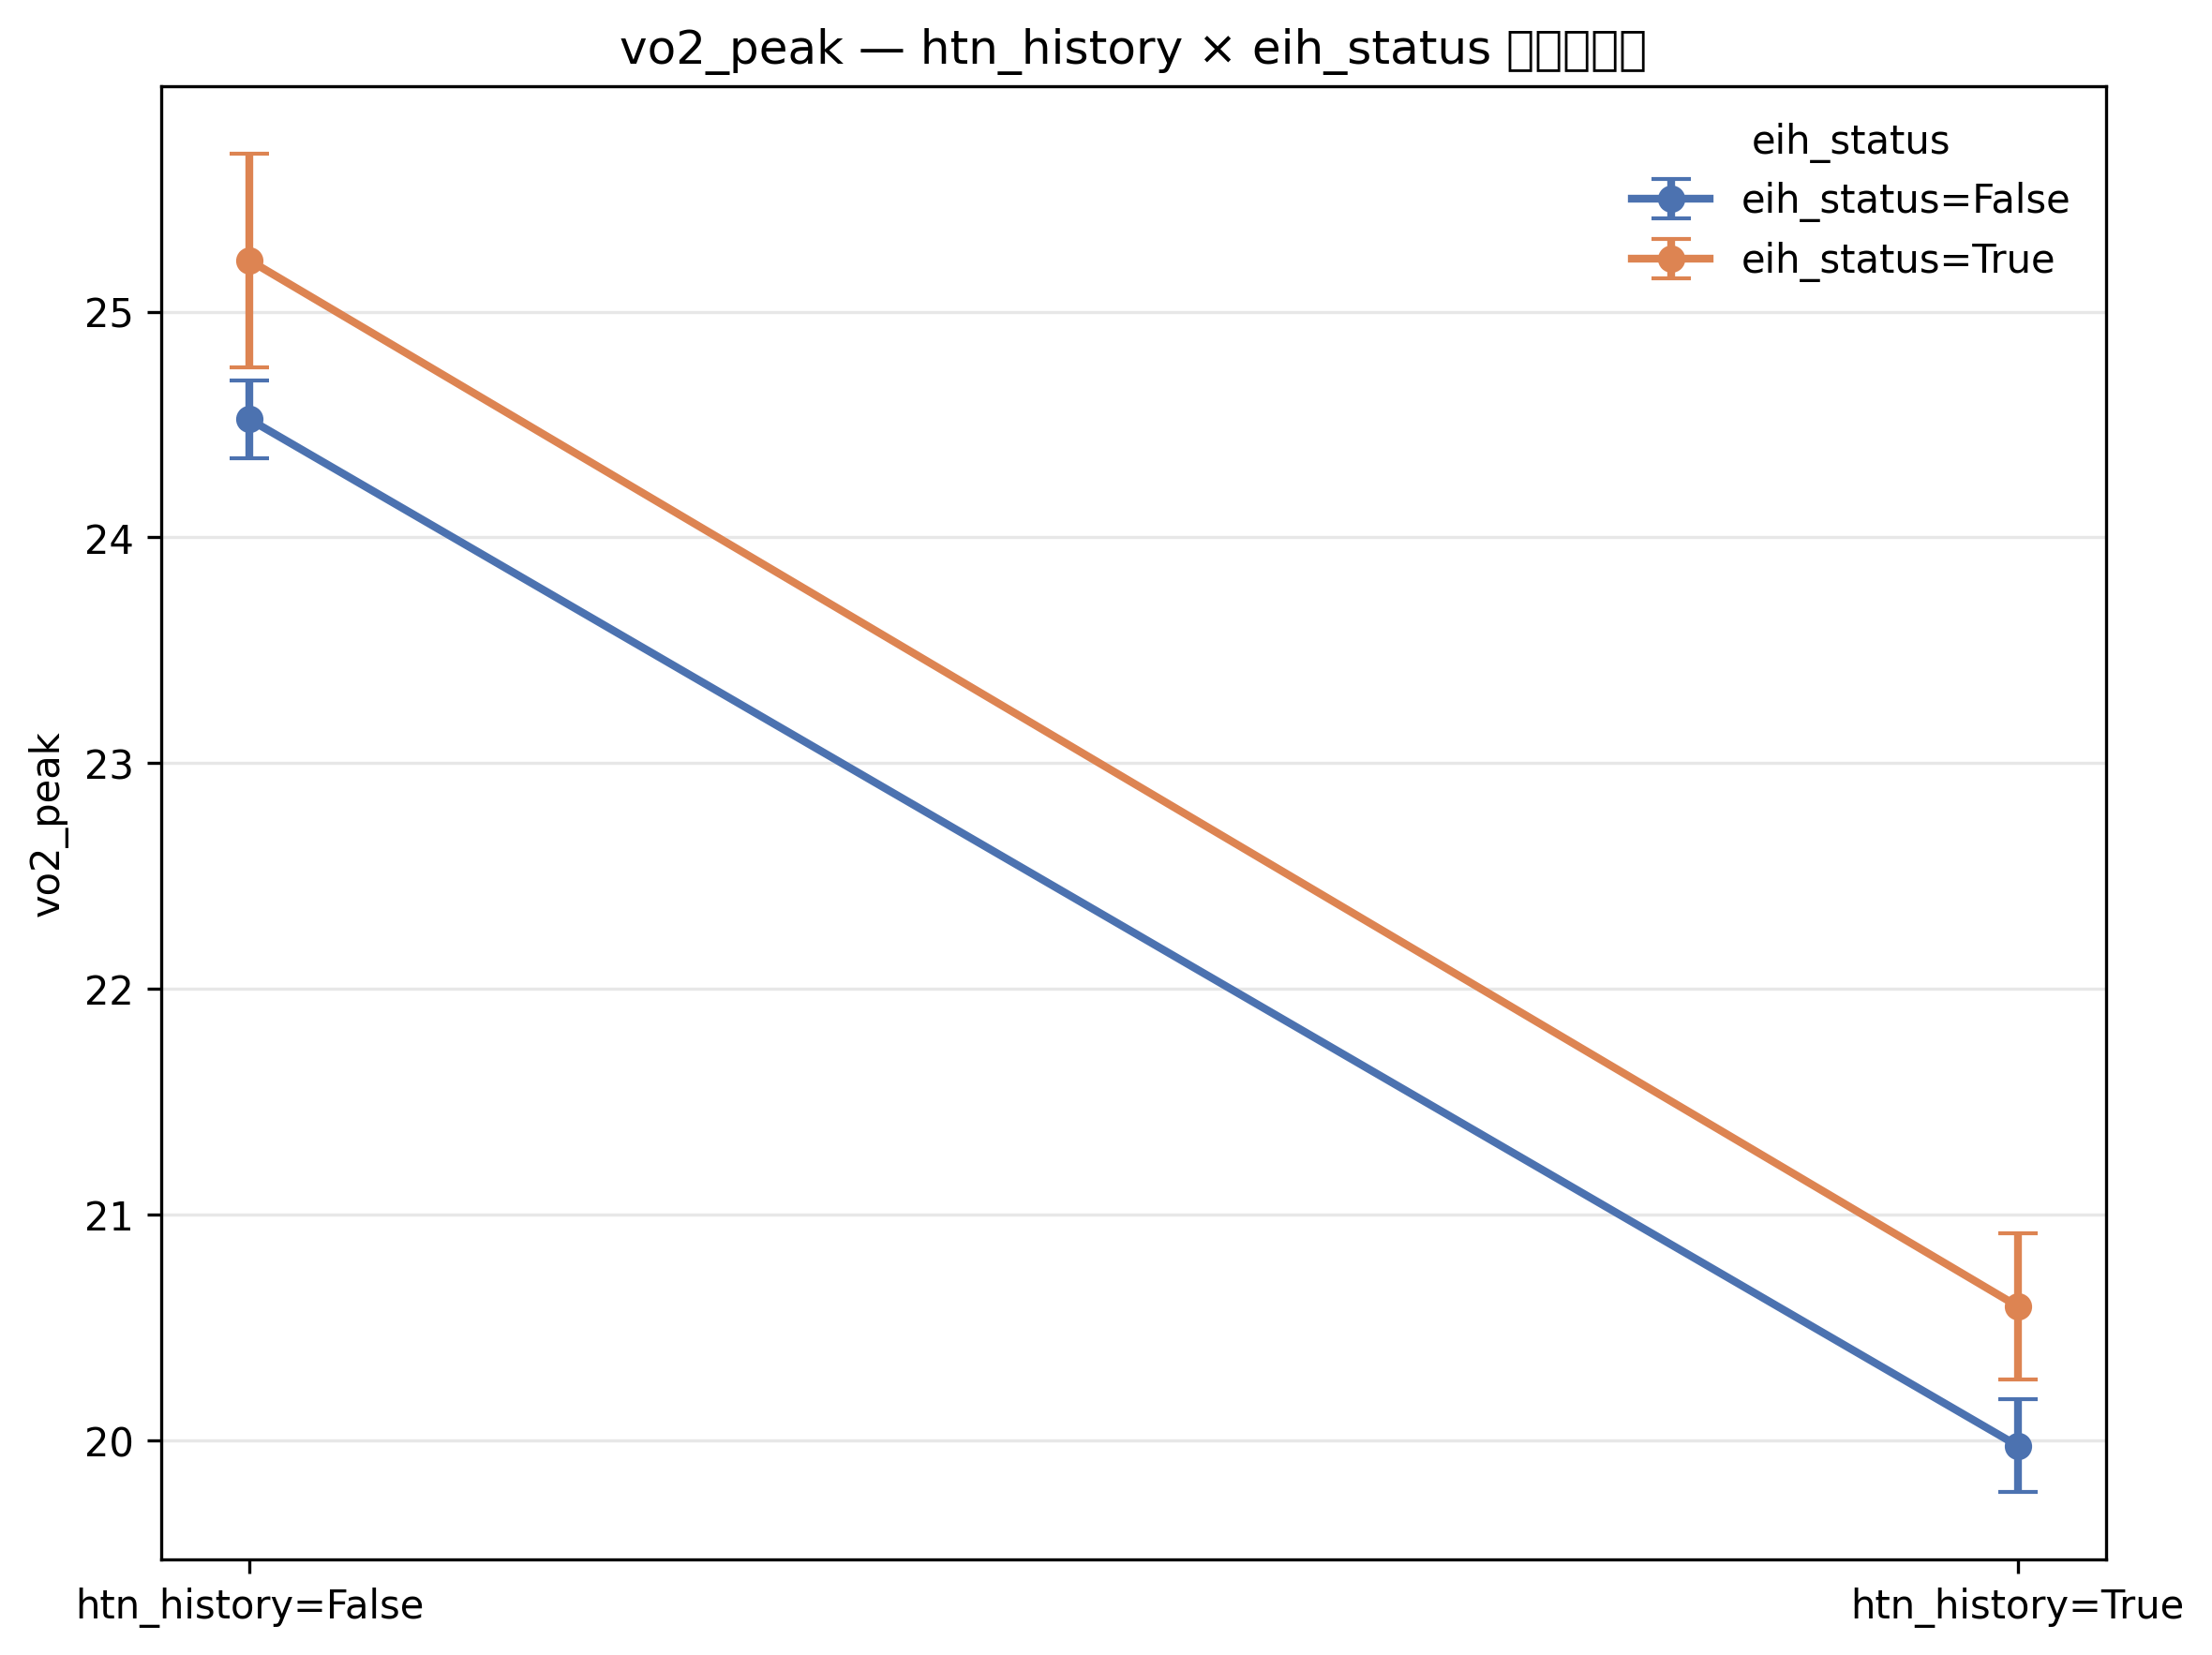
\includegraphics[width=0.85\textwidth]{figures/interaction_plots.png}
\caption{HTN$\times$EIH two-way interaction plots (VO$_2$peak group means).
CTRL vs.\ HTN groups differ significantly ($\eta^2$=0.084, medium effect);
EIH$+$/EIH$-$ groups within the same HTN stratum show similar VO$_2$peak,
with non-significant interaction ($p$=0.894).}
\label{fig:interaction}
\end{figure}

\begin{figure}[H]
\centering
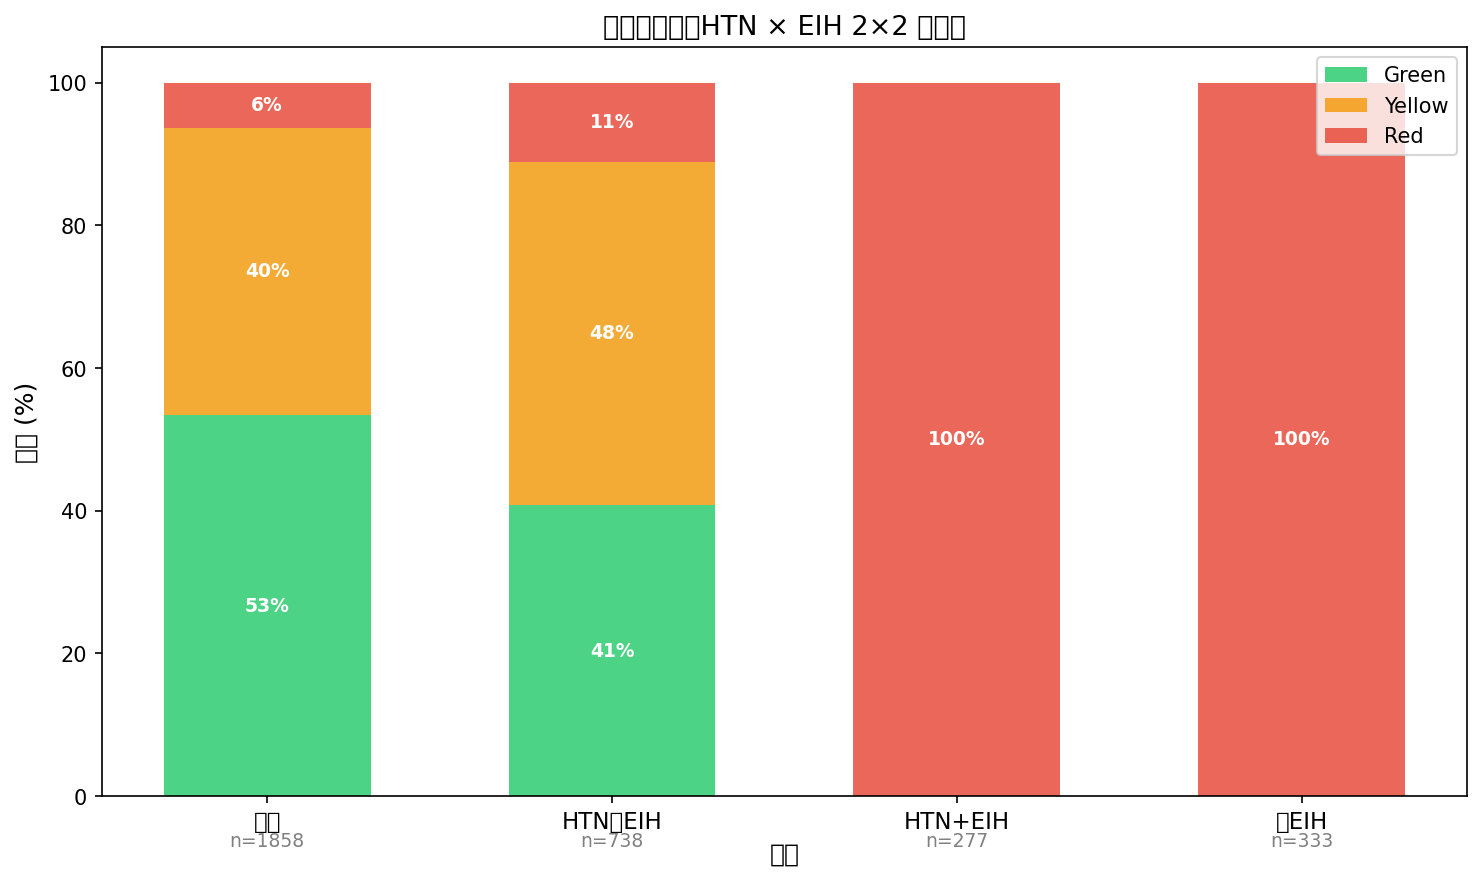
\includegraphics[width=0.85\textwidth]{figures/zone_distribution_stacked.png}
\caption{Safety zone distribution (Green/Yellow/Red) by HTN$\times$EIH 2$\times$2
cohort (stacked bar chart). EIH$+$ groups (HTN-EIH and EIH-Only) are
near-entirely Red (99.3\%/97.3\%), reflecting the EIH-Red axiom in P1 label definition.}
\label{fig:zone_dist}
\end{figure}

\begin{figure}[H]
\centering
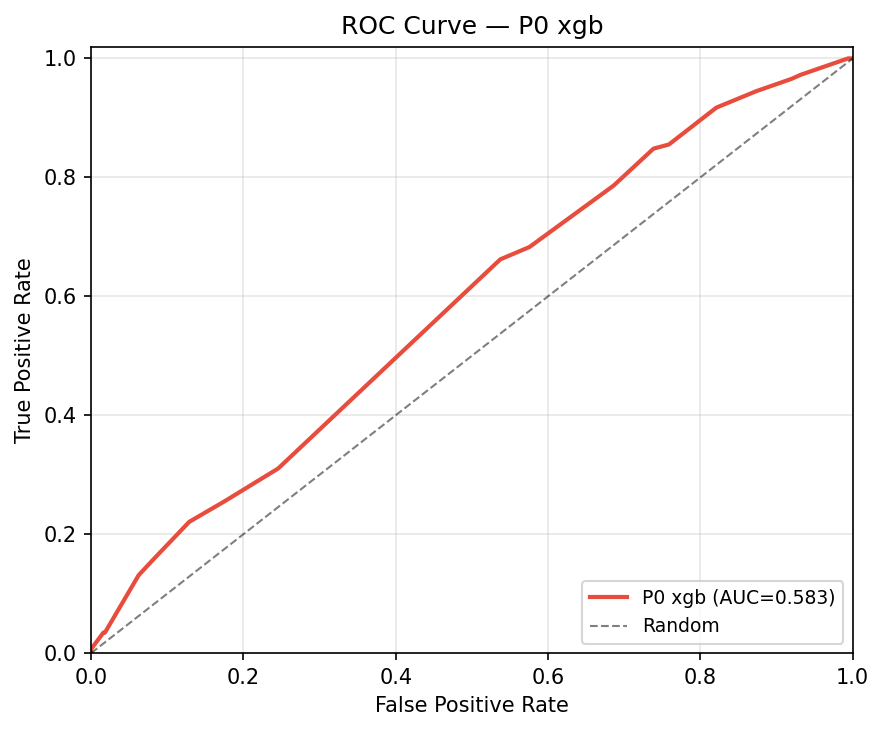
\includegraphics[width=0.65\textwidth]{figures/p0_roc.png}
\caption{P0 XGBoost ROC curve (no-BP variant, AUC=0.583). The curve near the
diagonal reflects the predictive limitation of summary-level data.}
\label{fig:p0_roc}
\end{figure}

\begin{figure}[H]
\centering
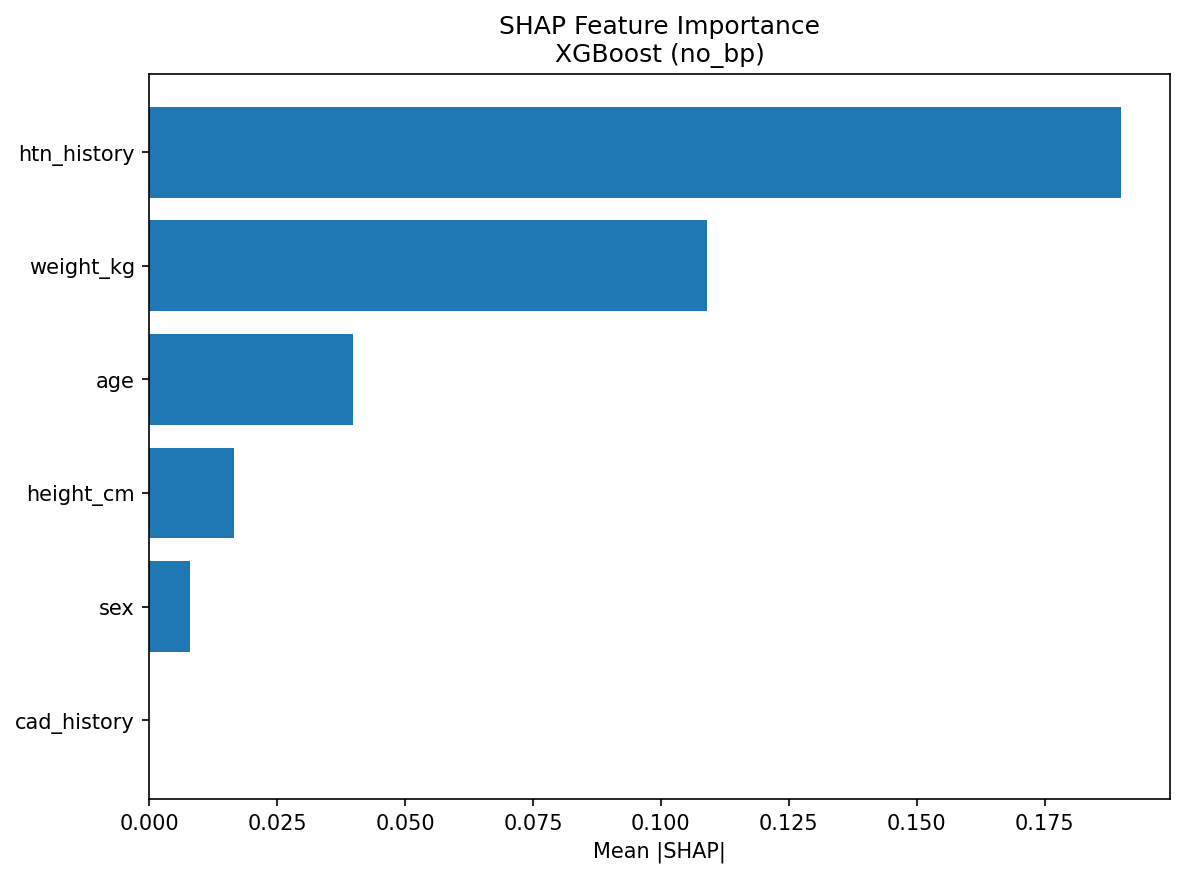
\includegraphics[width=0.85\textwidth]{figures/shap_p0.png}
\caption{P0 XGBoost SHAP global feature importance (no-BP variant).
Age and HTN history are the most important predictors.}
\label{fig:shap_p0}
\end{figure}

\begin{figure}[H]
\centering
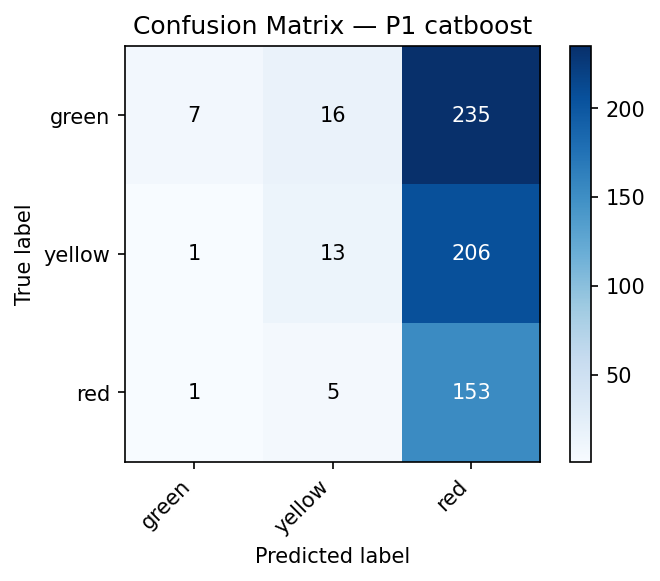
\includegraphics[width=0.65\textwidth]{figures/p1_cm_catboost.png}
\caption{P1 CatBoost best-model confusion matrix (F1$_\text{macro}$=0.499, $\kappa$=0.302).
Green recall 67.1\% (173/258); Red recall 30.8\% (49/159).}
\label{fig:p1_cm}
\end{figure}

\begin{figure}[H]
\centering
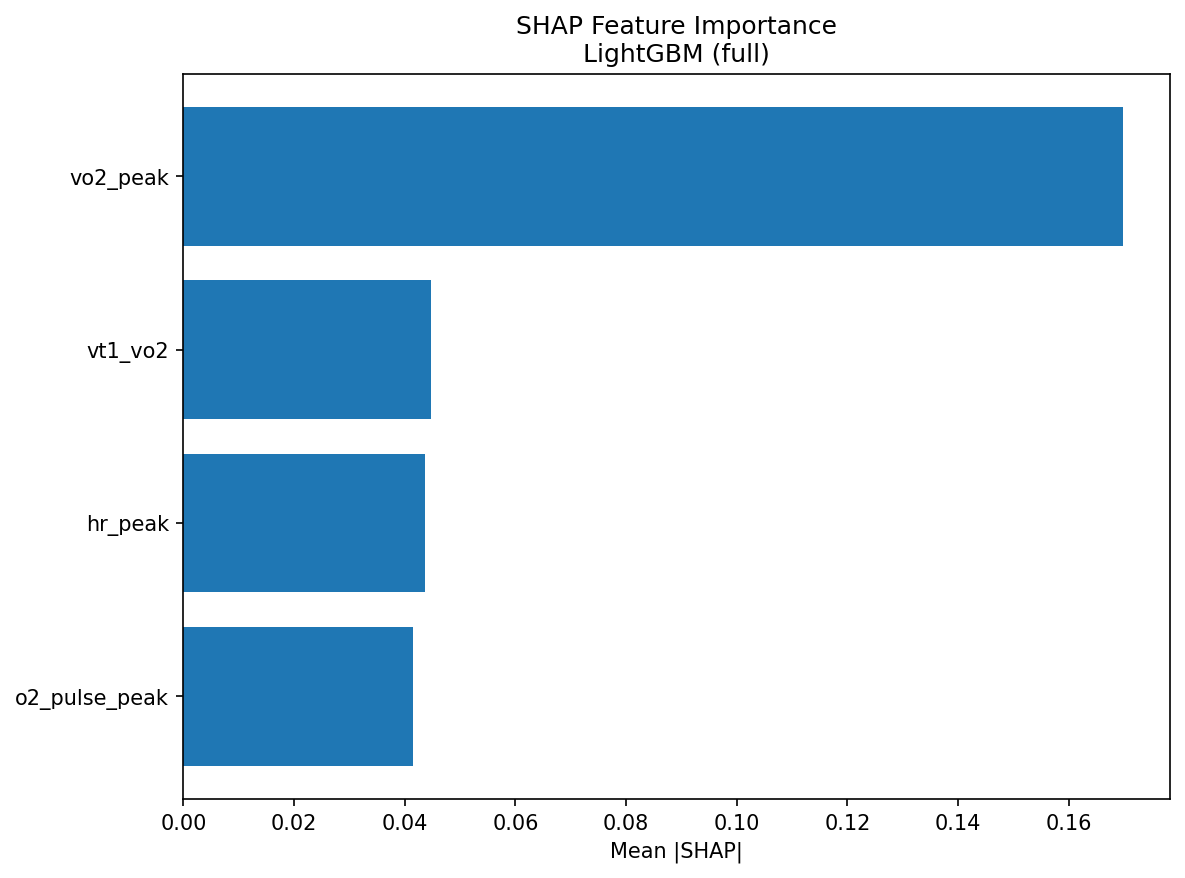
\includegraphics[width=0.85\textwidth]{figures/shap_p1.png}
\caption{P1 LightGBM SHAP global feature importance (full-sample variant).
VO$_2$peak and peak HR are the dominant classification features.}
\label{fig:shap_p1}
\end{figure}

\begin{figure}[H]
\centering
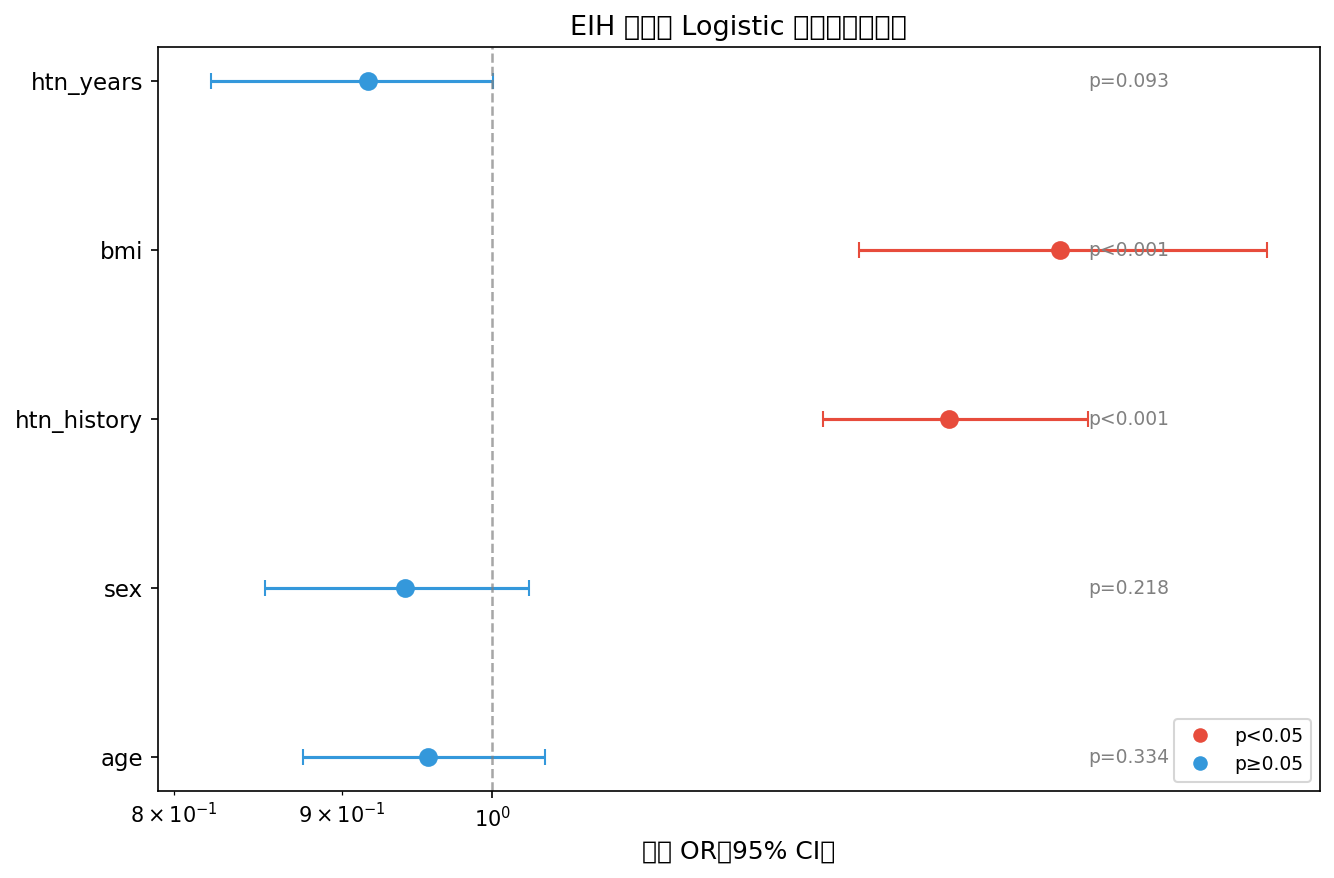
\includegraphics[width=0.65\textwidth]{figures/eih_forest.png}
\caption{Forest plot of EIH independent predictors (multivariable Logistic regression).
HTN history (aOR=1.44) and BMI (aOR=1.59) are the strongest independent predictors.}
\label{fig:eih_forest}
\end{figure}

\end{document}
